\chapter{System Architecture}

All systems, whether small or purposeful, must have an architecture clearly established so that their constituent parts may work smoothly and reliably together. As part of our analysis and design process, we considered several methods for structuring the system. We started with a simple architecture that includes the the core concepts and provides a clear, hopeful foundation for understanding the system’s operation. However, as we delved deeper into real-world requirements and constraints, we had to created a more complex architecture that more accurately reflected the issues and complexity of real-world deployment environments.

\section{Ideal Architecture}

As stated above we began by finding a simplified and hopeful architecture that on an ideal world would work, which would be the following:


\begin{figure}[H]
	\centerline{
		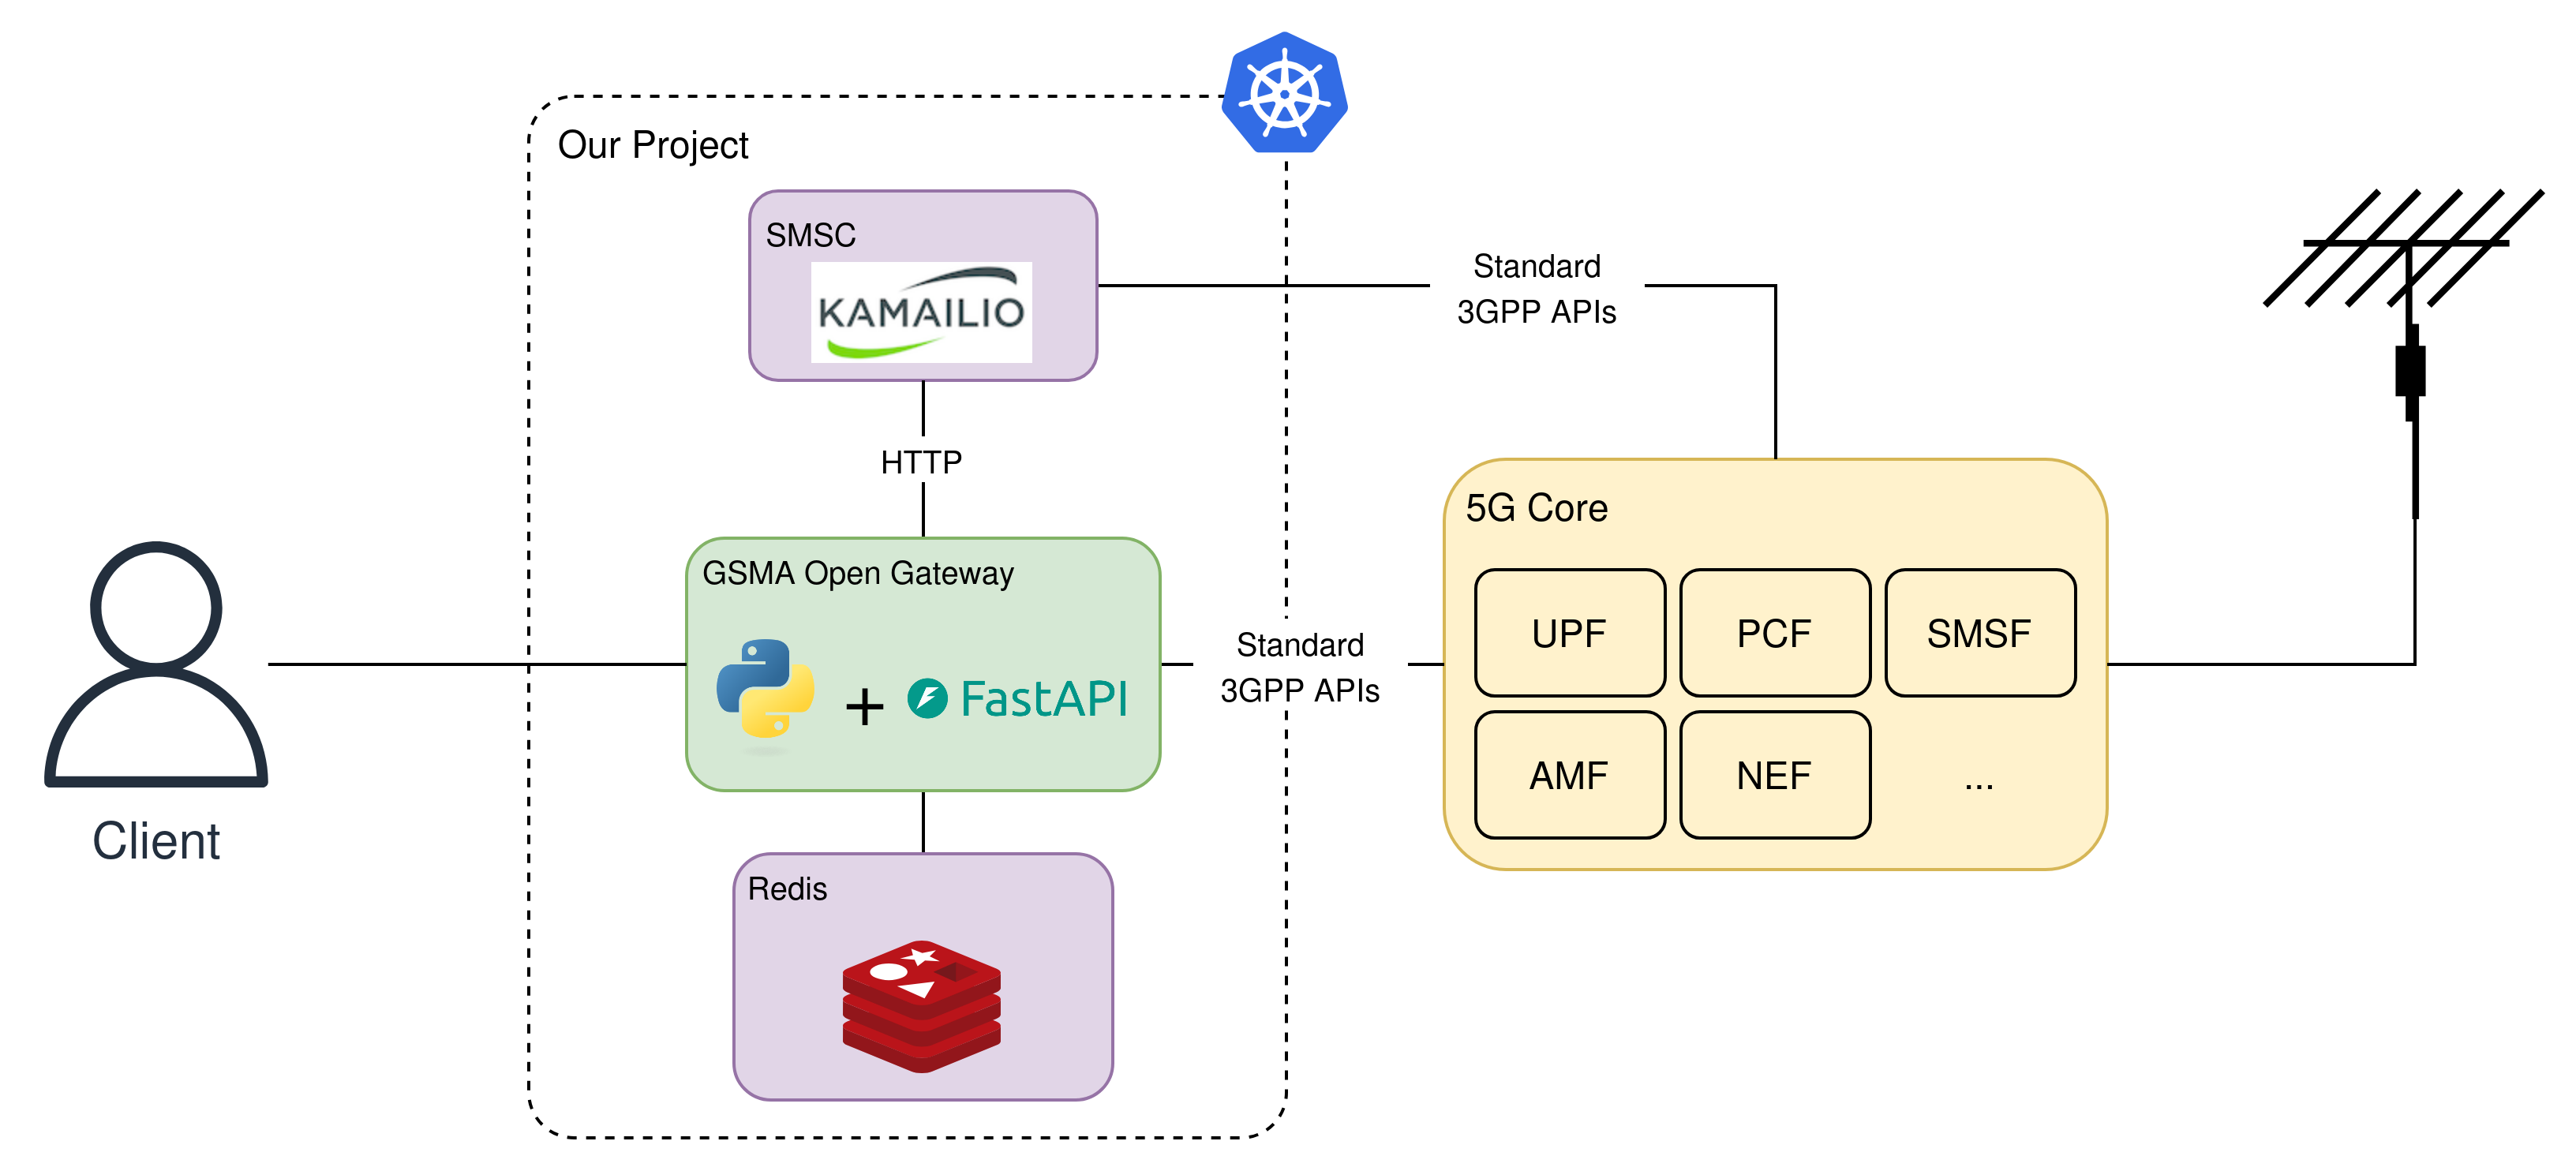
\includegraphics[width=15cm]{figs/IdealArchitecture.png}
	}
	\caption{Project's Ideal Architecture}
\end{figure}

Here the existing infrastructure would provide a 5G core that is compliant with the 3GPP standards, providing APIs to interact with the relevant network functions that would be consistent from core to core. Furthermore, Short Message Services (SMS) would be available and exposed programmatically for use.

In this scenario, our work would be relatively simple. We would need to deploy an SMS Centre (SMSC) that would connect to the standards compliant core and handle storing and forwarding SMSs while also providing an interface to do so programmatically to our service. This component, while not developed by us, would be configured, packaged and deployed by us.

Then the GSMA Open Gateway would be developed by us and talk to the 5G Core and SMSC using the standardized interfaces. This would allow our project to talk to any core as long as they followed the standards, increasing the portability of our solution. This component would be what the vertical customers would interact with, and would be assisted by a Redis database to keep track of some state between requests.

All this work would be packaged through the use of Helm Charts that would allow the deployment of this solution to a Kubernetes cluster. This would further allow offering our solution as a service, as the chart could be installed multiple times with tweaked values for each client.

However, as stated before this ideal architecture was not able to be achieved due to some complexity of the tools provided, so we had to reach a real architecture, that would take into account these problems.

\section{Real Architecture}

However, as we have seen before, reality isn't as simple. There are some problems with our idealized architecture:
\begin{itemize}
	\item Not all cores are standards compliant. Many of them provide only proprietary APIs and some don't even provide APIs and only provide graphical or command line interfaces.
	\item Not all functionality is supported by the cores. In a real world scenario, the gateway would simply not offer some services that were dependent on these. However, as we are interested in exploring what kind of applications could be offered through the GSMA Open Gateway API, emulating the missing functionality is more advantageous to us.
	\item The core we were provided had no integration with any telephony services, which would not allow us to send SMS messages, an important action in order to implement the SMS OTP API.
\end{itemize}

To address these problems, we reached the following architecture:

\begin{figure}[H]
	\centerline{
		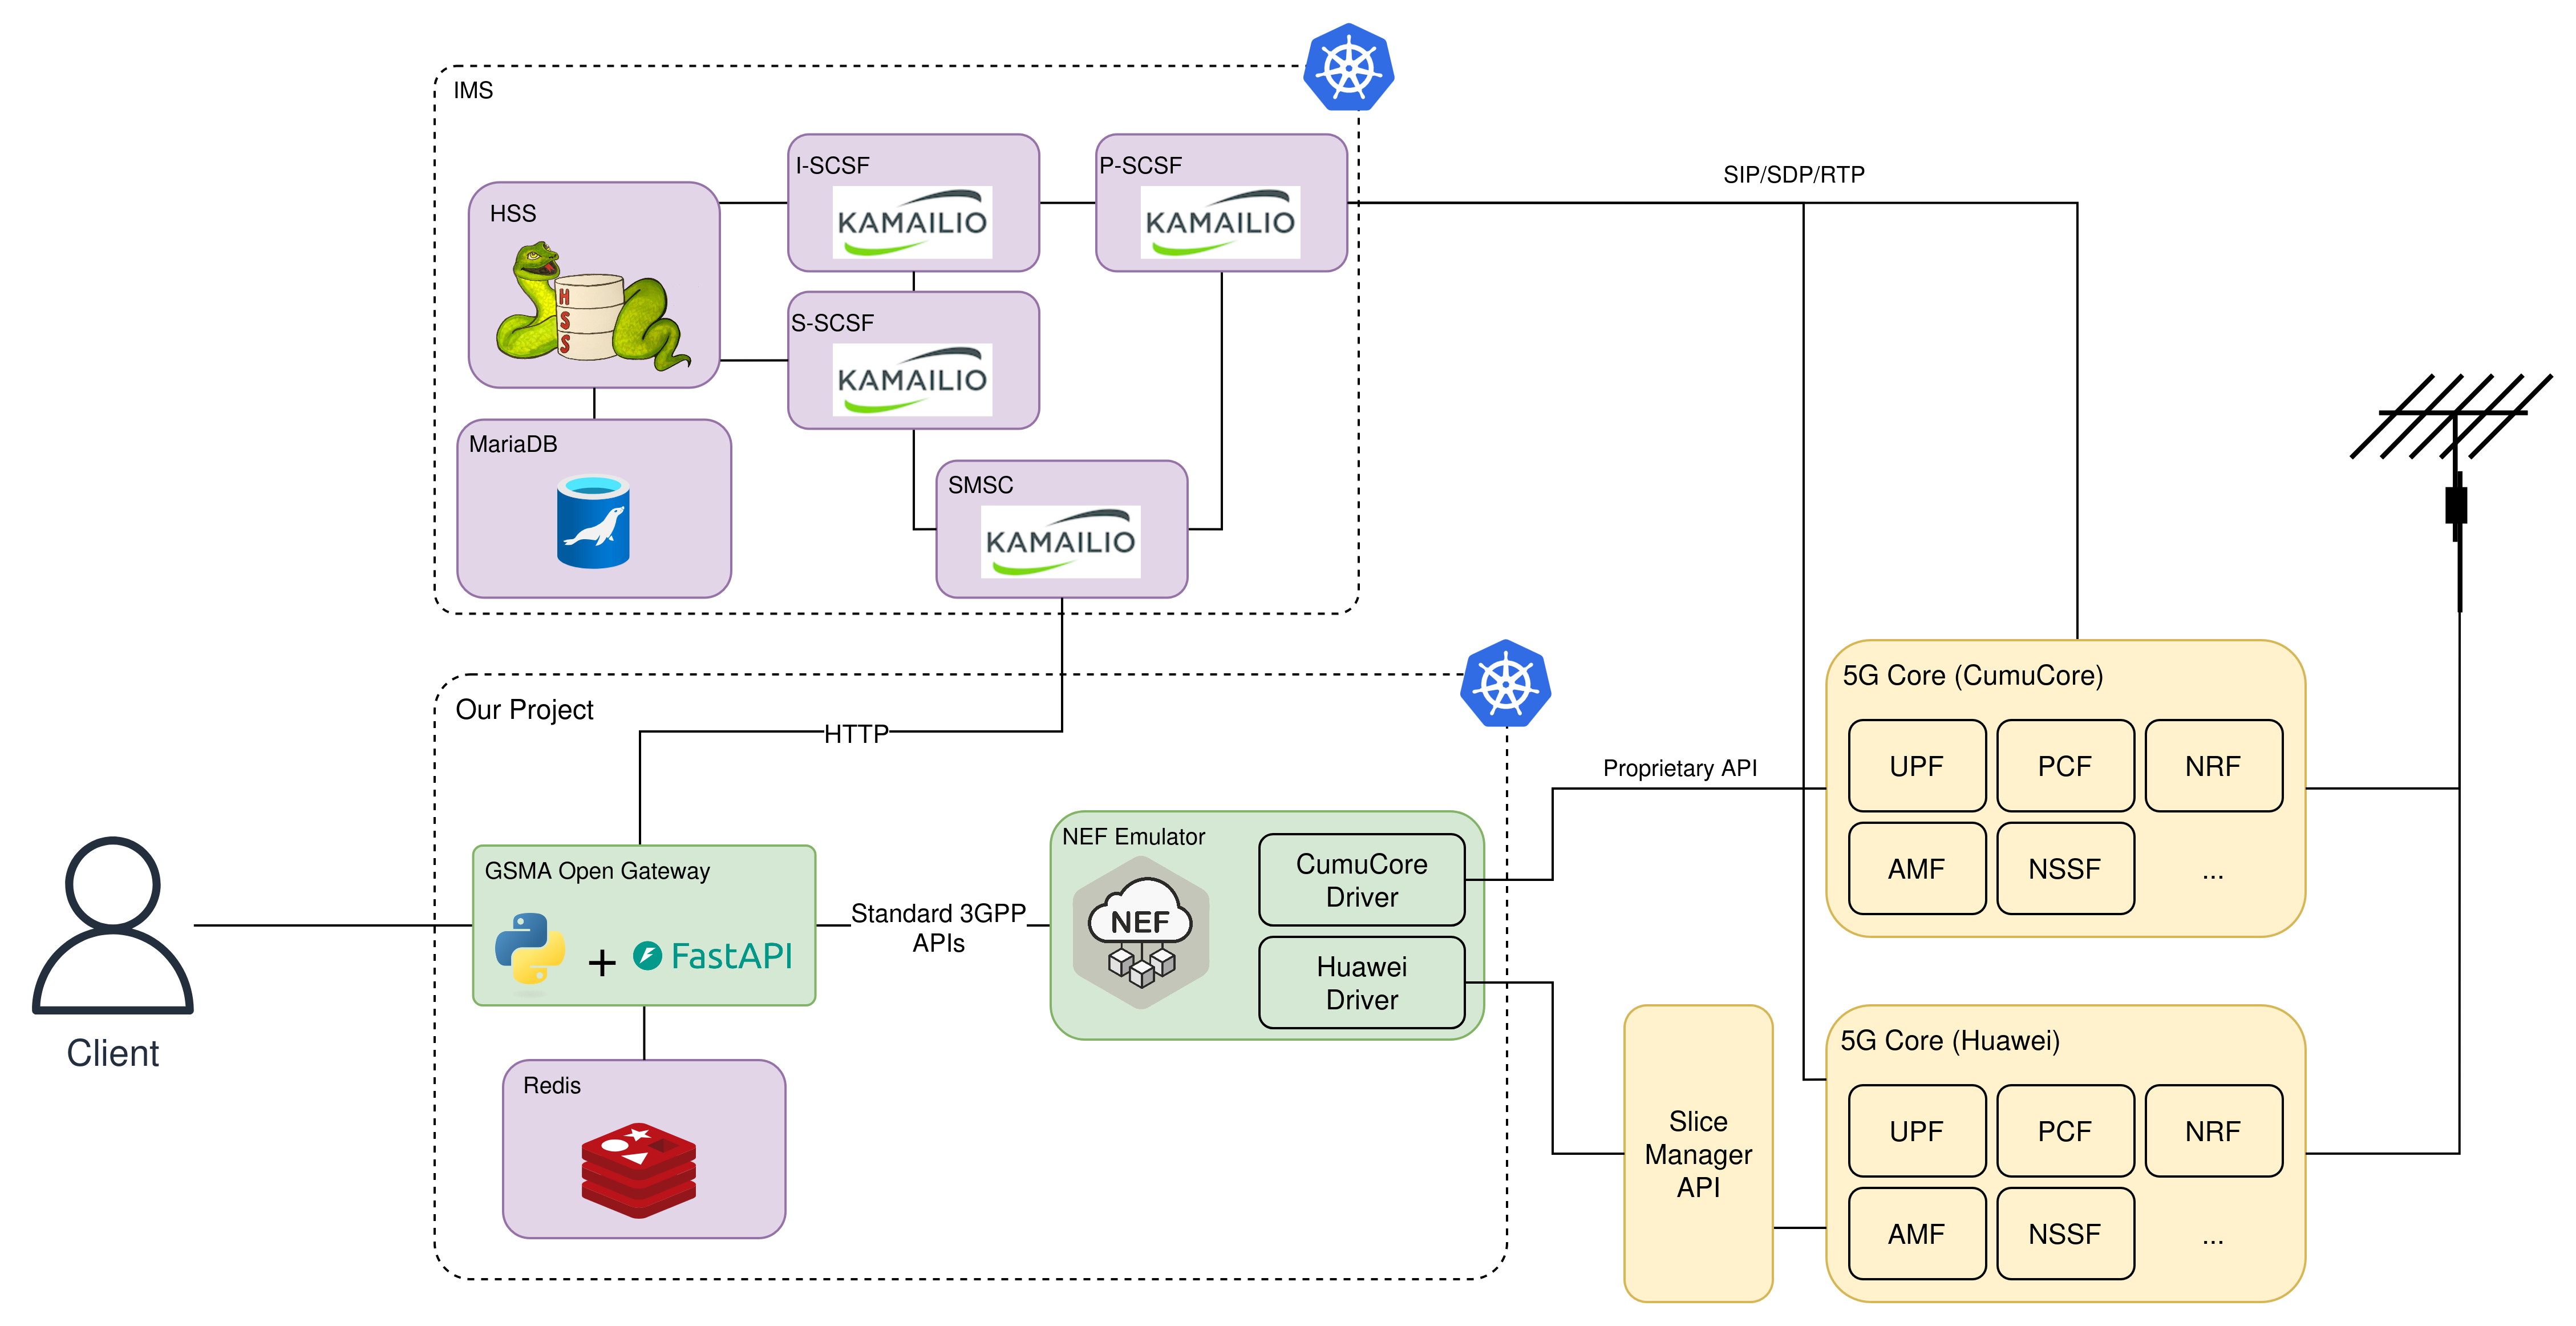
\includegraphics[width=15cm]{figs/RealArchitecture.png}
	}
	\caption{Project's Ideal Architecture}
\end{figure}

Now, a NEF Emulator will be deployed to emulate functionality that isn't provided by the cores currently available at IT Aveiro, mainly location APIs. Furthermore, it will also be used to communicate with the different cores through different drivers, each for their respective core, this means that this emulator will be used as an actual NEF. One could interface standards compliant cores, others could support proprietary APIs exposed by the cores (as seen in the case of CumuCore), and finally there could be implementations that talk to middlewares that wrap the interfaces of cores that don't have APIs (as is the case for the Huawei implementation).

Moreover, instead of the gateway communicating directly to the core, it would communicate with 3GPP compliant interfaces presented by the NEF Emulator.

Finally, to provide telephony services an IP Multimedia Subsystem (IMS) will be deployed. This set of components allows the user equipment (mobile phones) to place calls and exchange messages with the aid of the SMSC. The IMS comprises multiple Call Session Control Functions (CSCF) that each take on a different role: Proxy (P-CSCF), Interrogating (I-CSCF), and Serving (S-CSCF). Additionally, a Home Subscriber Server (HSS) based on PyHSS with a MariaDB is required by the CSCFs for authentication and tracking of clients. All of this infrastructure will be configured and deployed by us as a Helm Chart. The inclusion of IMS is required because the cores don't provide these services by themselves, and we intend to implement the OTP SMS APIs, which require the sending of SMSs.

As was the case in the ideal architecture, all components of our project will be packaged in a Helm Chart (one for our project specific components and another for the IMS), to allow deployment on a Kubernetes cluster. As stated before, this also opens the door to offering everything as a service.


